\documentclass[a0,portrait]{a0poster}


\usepackage{multicol}
\columnsep=100pt
\columnseprule=3pt
\usepackage{fancybox}
\usepackage[svgnames]{xcolor}
\usepackage{wrapfig}
\usepackage{epsfig}
\usepackage{pdfpages}
\usepackage{cite}
\usepackage{color}
\usepackage{colortbl}
\usepackage[cmex10]{amsmath}
\usepackage{amssymb}
\usepackage{soul}
\usepackage{amsfonts}
\usepackage[normalem]{ulem}
\usepackage{booktabs}
\usepackage{color}
\usepackage{placeins}
\usepackage{upgreek}
\usepackage{subfigure}
\usepackage{subcaption}
\usepackage[utf8]{inputenc}
\usepackage[framemethod=tikz]{mdframed}

\usepackage[export]{adjustbox}
\usepackage{epstopdf}
\usepackage{graphicx,float} 
\usepackage{booktabs} 
\usepackage[font=small,labelfont=bf]{caption} 
\usepackage{amsfonts, amsmath, amsthm, amssymb}
\usepackage{wrapfig}
\usepackage{titlesec} 

\newcommand{\ds}{\displaystyle}
\newcommand {\bo}[1]{\textbf{#1}}
\newcommand{\pa}[1]{\left({#1}\right)}
\newcommand{\co}[1]{\left[{#1}\right]}
\newcommand{\ch}[1]{\left\{{#1}\right\}}

\definecolor{RITOrange}{rgb}{1,0.321,0}
\definecolor{HUPurple}{rgb}{0.36078, 0.145098, 0.407843}

% \pdfpagewidth 48.0in
% \pdfpageheight 96.0in


% \titleformat{\section}{\color{white}\normalfont\Large\bfseries}{\color{white}\thesection}{1em}{\colorbox{HUPurple}}{}
\titleformat{\section}{\color{HUPurple}\normalfont\Large\bfseries}{}{}{}{}

\setlength{\columnseprule}{0pt}

\begin{document}

\begin{minipage}[b]{0.33\linewidth}
\raggedright

\includegraphics[height=3cm,valign=t]{assets/logos/ccrg-logo.png}
\end{minipage}
%
\begin{minipage}[b]{0.33\linewidth}
\centering

\includegraphics[height=3cm,valign=t]{assets/logos/full_bright_logo.pdf}
\end{minipage}
% 
\begin{minipage}[b]{0.33\linewidth}
\raggedleft

\includegraphics[width=3cm,valign=t]{assets/logos/RIT_logo.pdf}
\end{minipage}\\

\vspace{3cm}
\begin{minipage}[h]{0.98\linewidth}
\centering \huge \color{HUPurple} \textbf{GWKokab: An Implementations to Identify the Properties of Multiple Population of Gravitational Wave Sources} \color{Black}\\ % Title
\Large \textbf{Meesum Qazalbash\textsuperscript{1}, Muhammad Zeeshan\textsuperscript{2}, and Richard O'Shaughnessy\textsuperscript{2}}\\ % Author(s)
\normalsize \textsuperscript{1} Habib University, Karachi, Pakistan,\textsuperscript{2} Rochester Institute of Technology, New York, USA \\ %[-0.5cm] % University/organization
% email@email.com\textsuperscript{1}, email@email.br\textsuperscript{2} and email@email.com\textsuperscript{3}\\
\end{minipage}
\vspace{0.5cm}


\section*{Abstract}

Gravitational wave events provide crucial insights into the population properties of compact binaries. This work introduces GWKokab, a JAX-based framework designed for flexible model building by combining simple components with independent rates for each subpopulation. To validate its robustness, we generate a synthetic population consisting of a spinning eccentric sub-population modeled with a power-law distribution and circular sub-populations modeled with a multi-source model comprising one power-law and three Gaussians. Our framework successfully recovers the injected parameters while significantly reducing computational costs. In addition, we demonstrate selected science applications, including the recovery of eccentric injections and the reproduction of key results from previous studies. GWKokab also enables the study of hierarchical mergers by analyzing spin signatures in sub-populations. The publicly available code is expected to facilitate the subpopulation analysis of future gravitational wave events with improved computational efficiency.



\begin{multicols}{3}

\section*{Reproduction: Eccentricity Matters}

\begin{frame}

\begin{figure}[H]
    \centering
    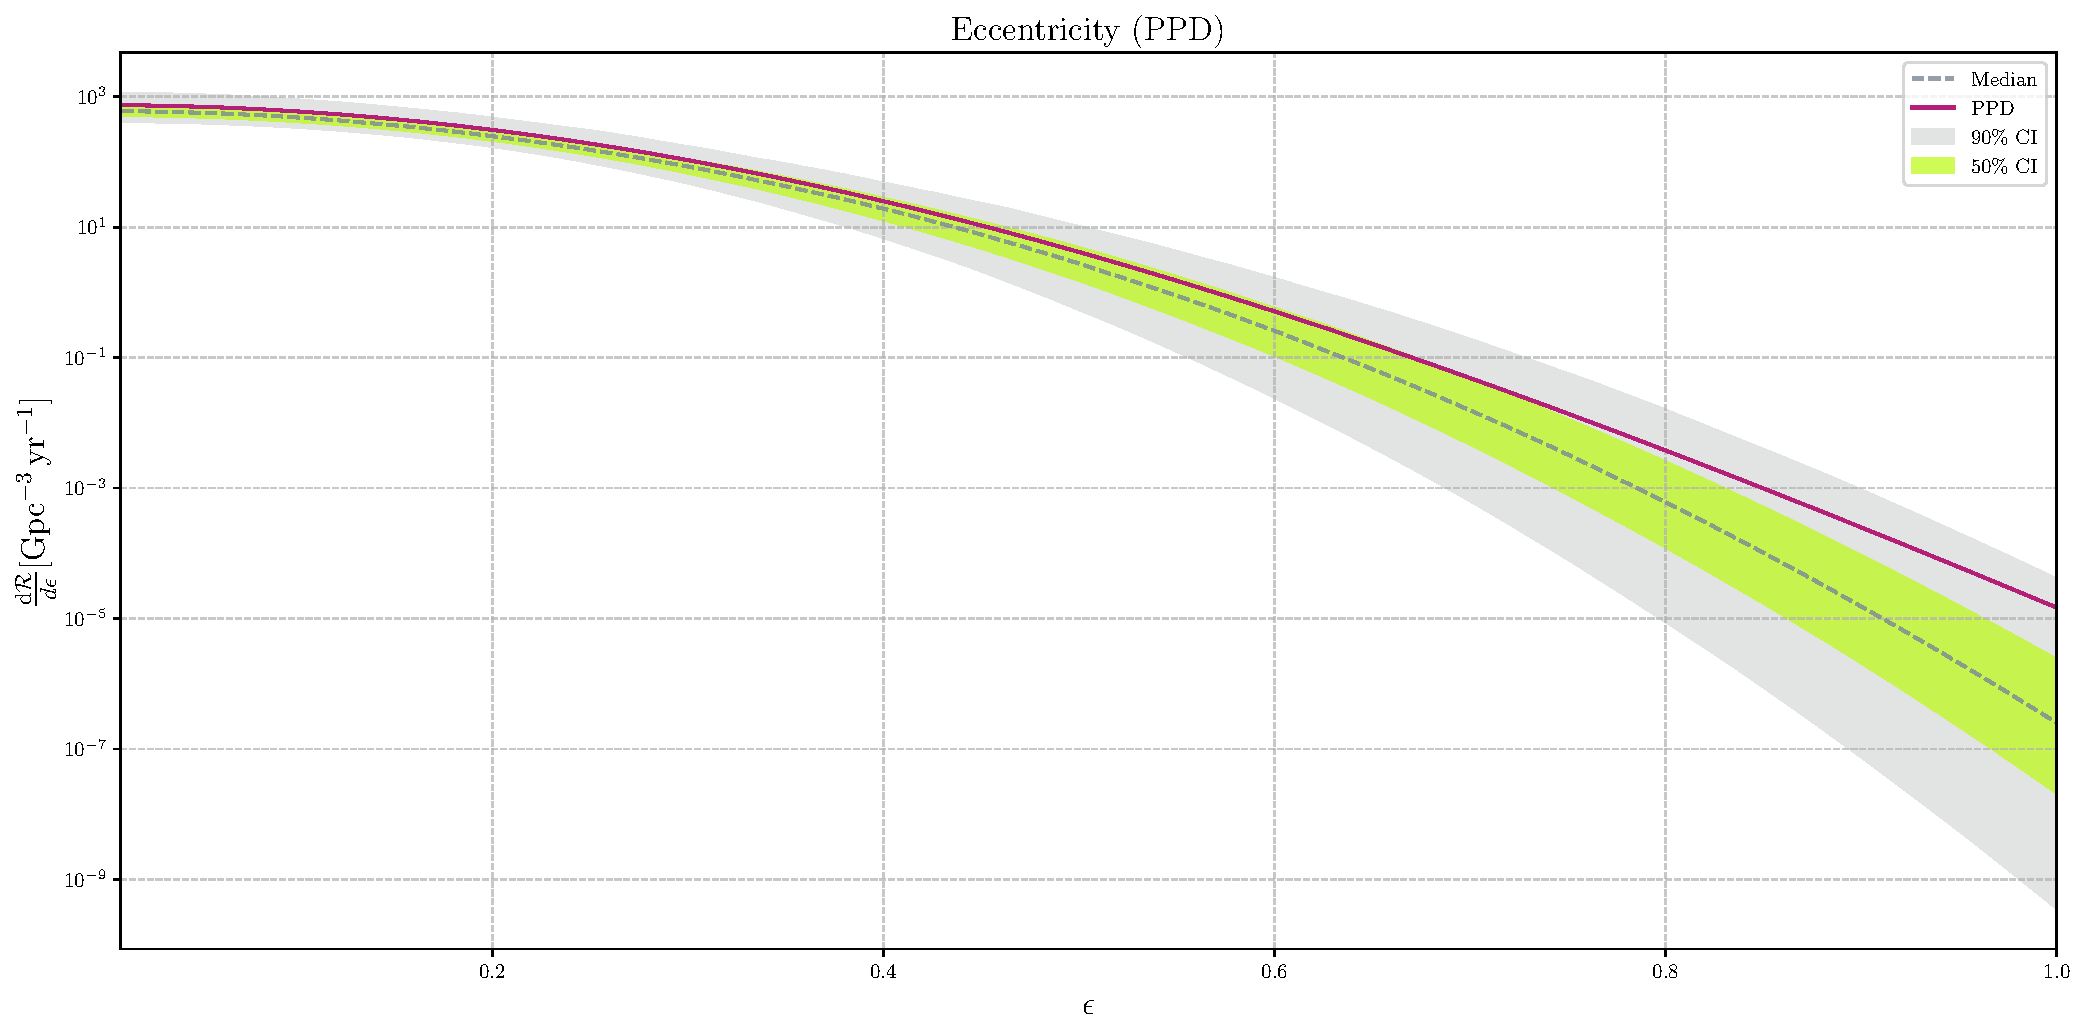
\includegraphics[width=0.7\linewidth]{assets/plots/rate_ecc_ppd_plot.pdf}
    \caption{Posterior Predictive distribution of Eccentricity}
    \label{fig:ppd-ecc}
\end{figure}

\begin{figure}[H]
    \centering
    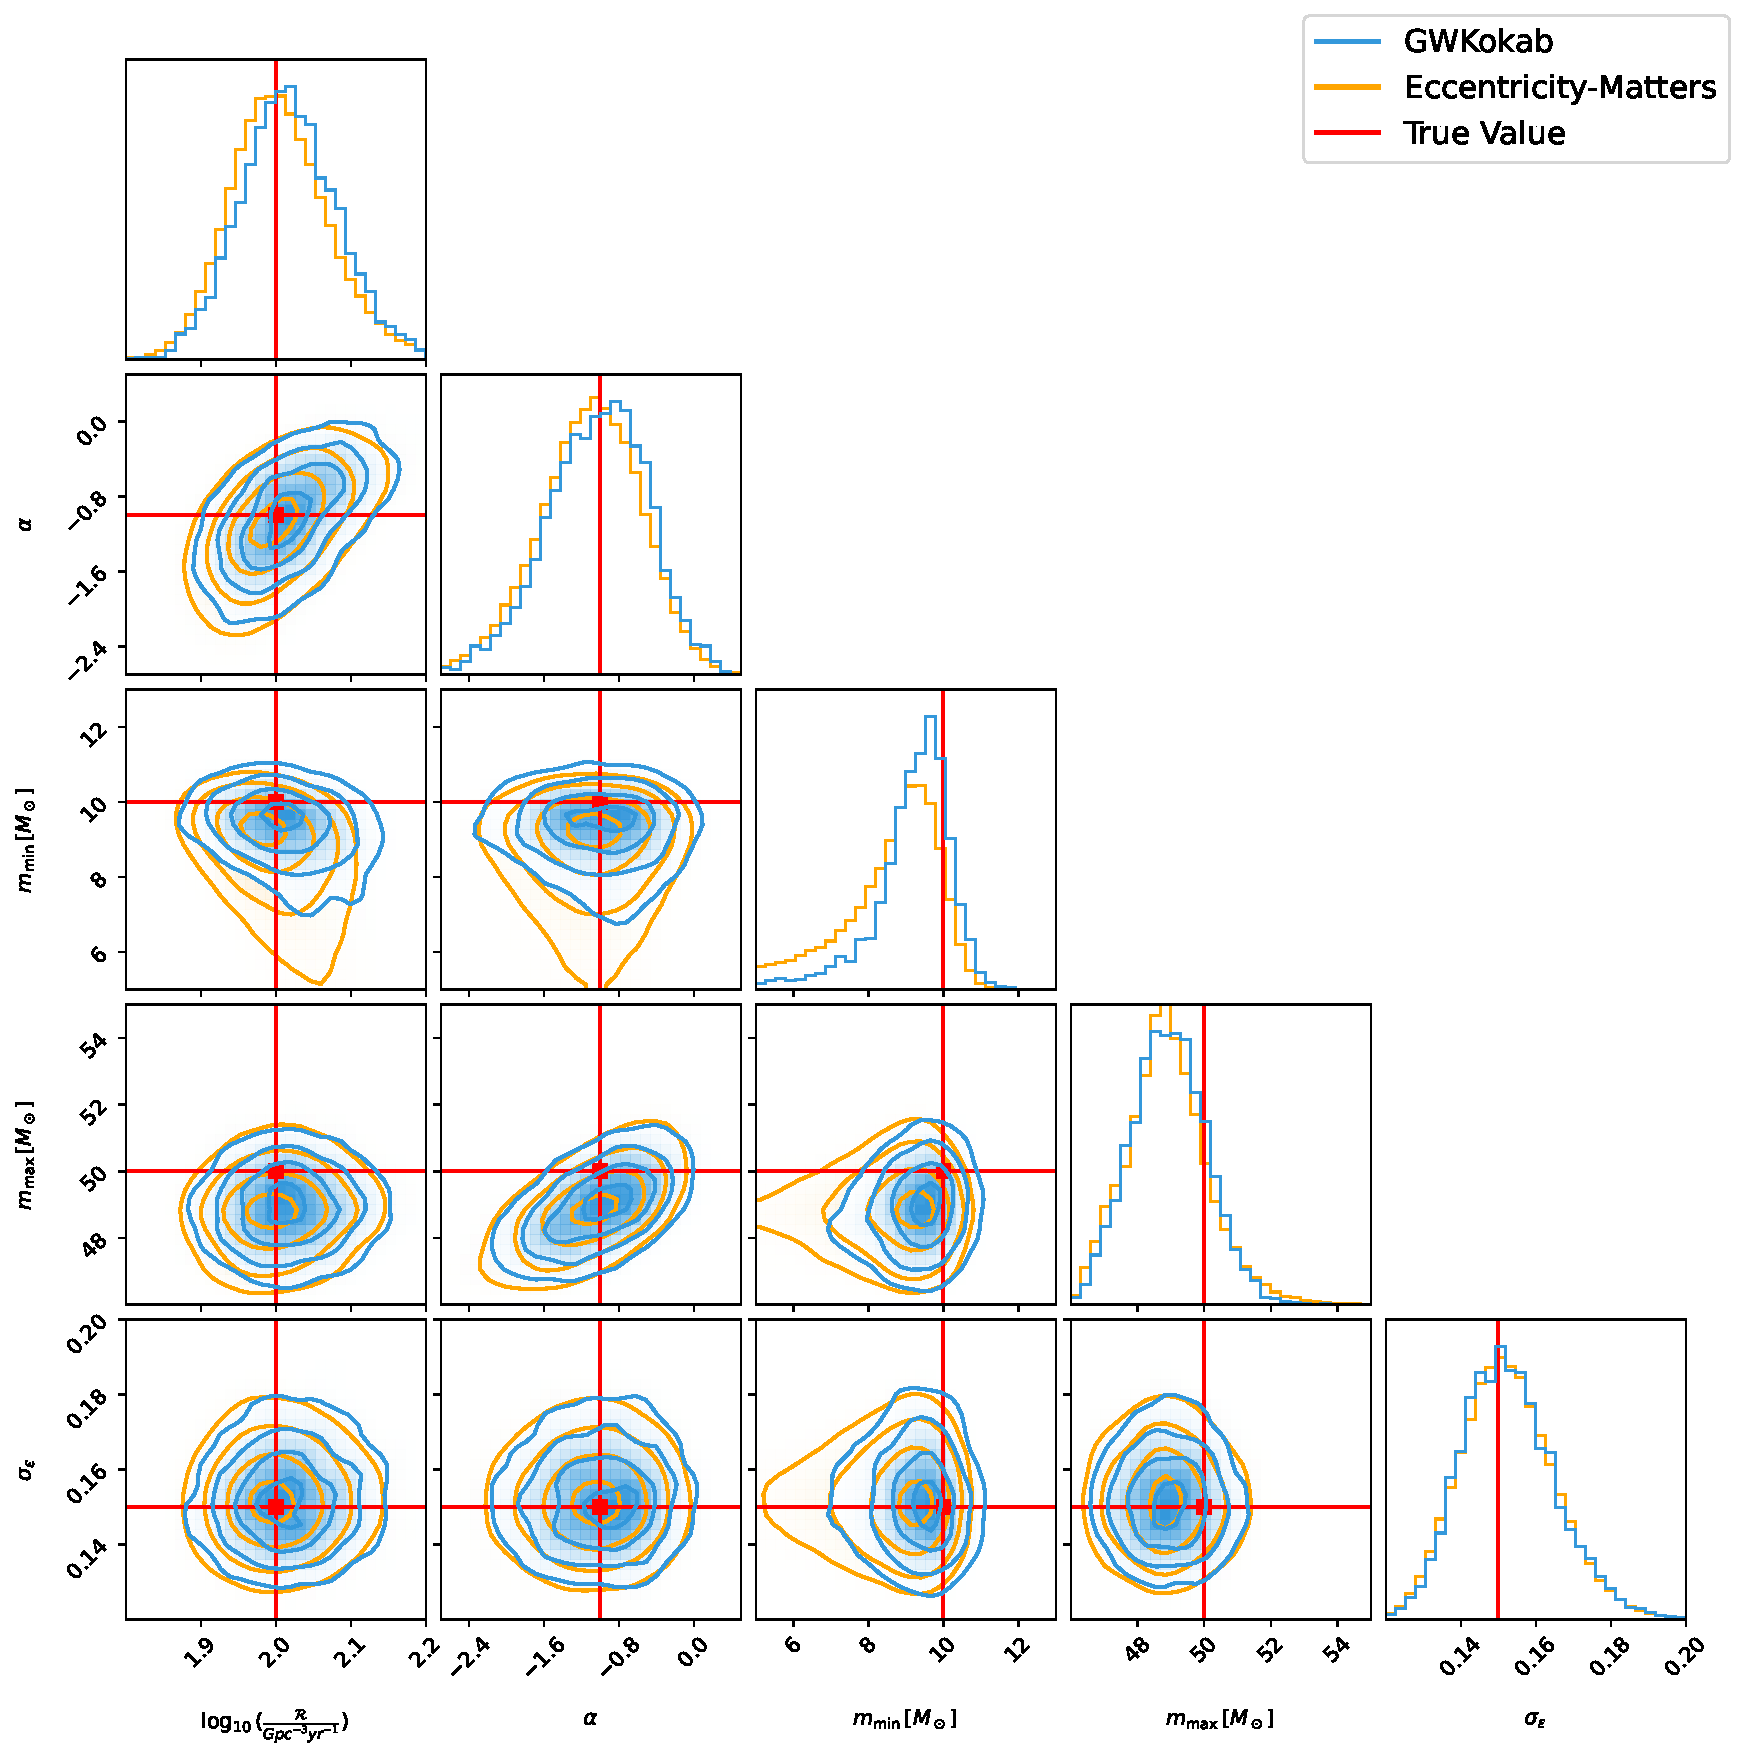
\includegraphics[width=0.7\linewidth]{assets/plots/normalized_ecc_data.pdf}
    \caption{Reproduction of published results at 98\% lesser computational cost using the same data generated by Ecc-Matters code.}
    \label{fig:ecc_matters_reproduction}
\end{figure}

\end{frame}

\columnbreak


\section*{Eccentric Spinning Population}

\begin{frame}

\begin{figure}[H]
    \centering
    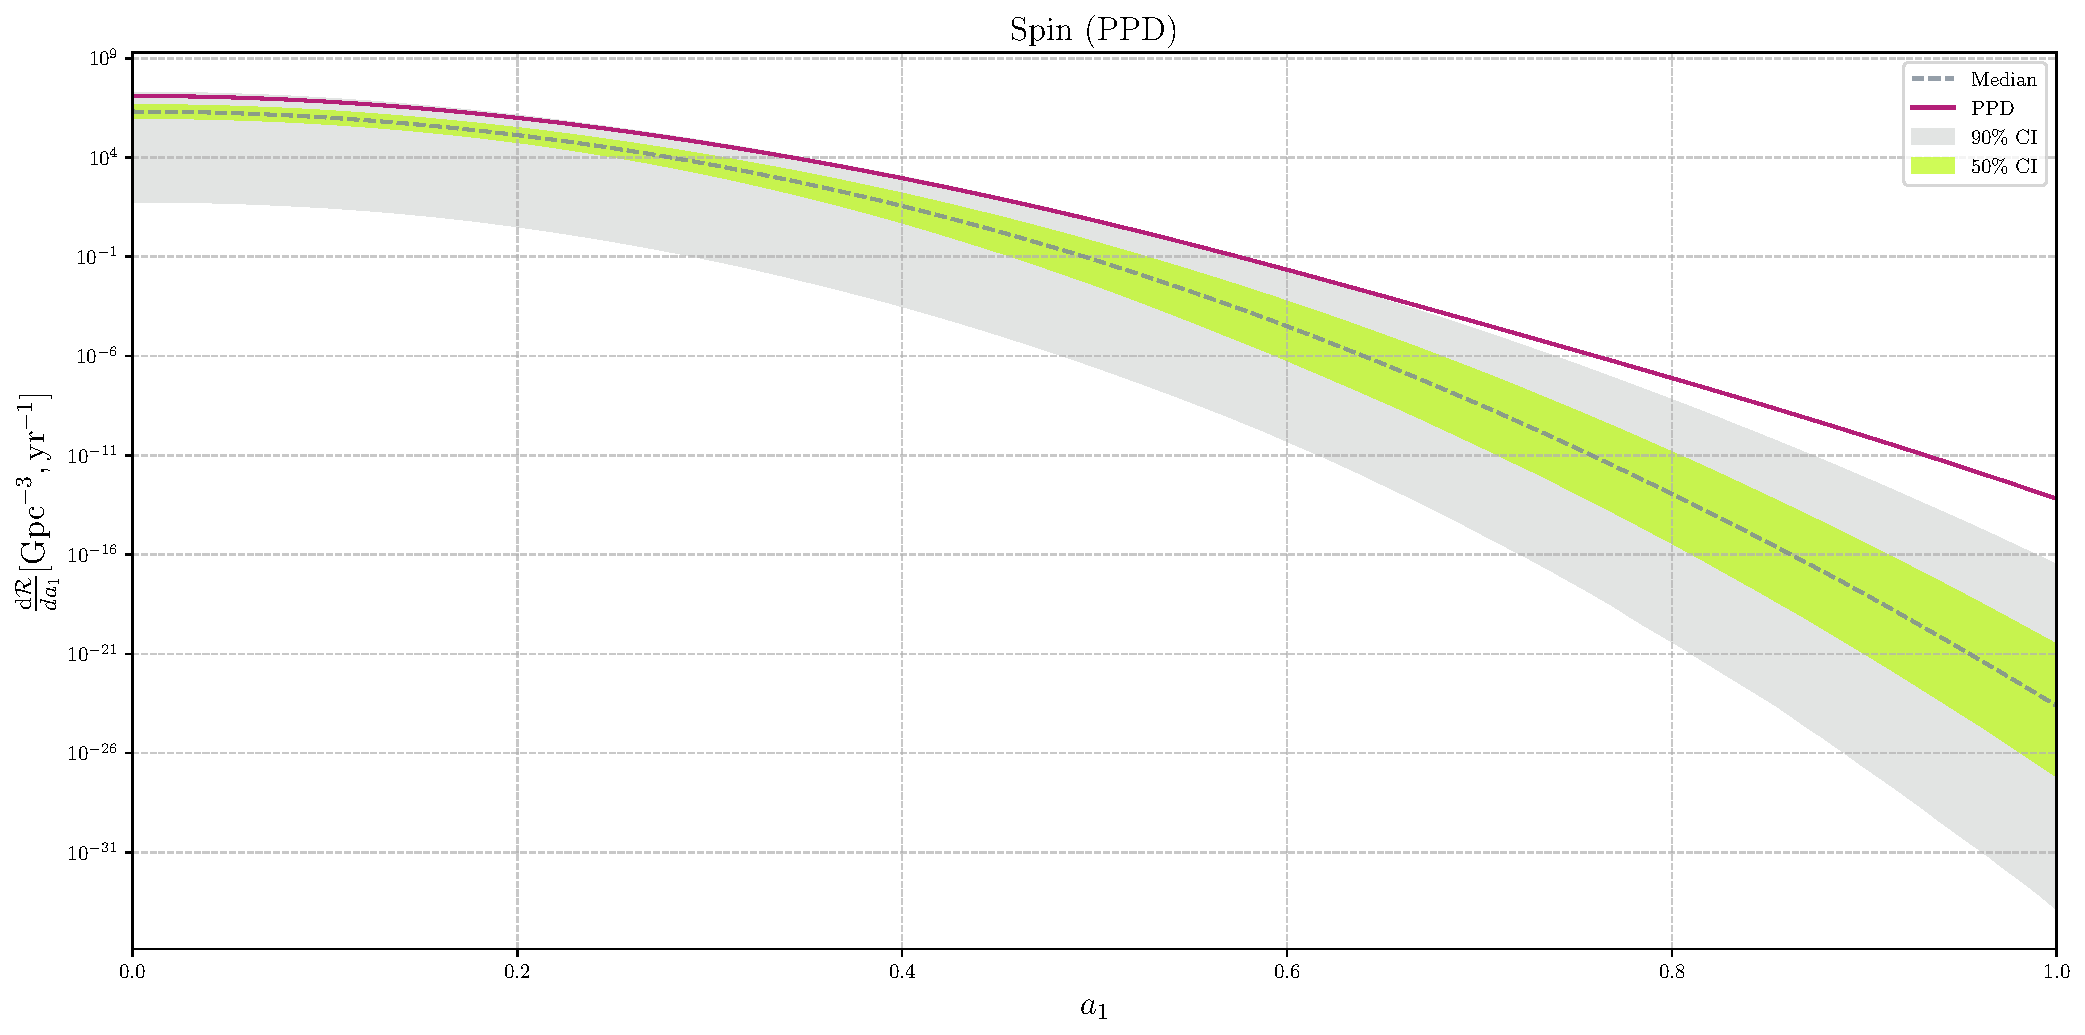
\includegraphics[width=0.7\linewidth]{assets/plots/rate_a_1_ppd_plot.pdf}
    \caption{Posterior Predictive Distribution of Primary Spin Magnitude}
    \label{fig:ppd-a1}
\end{figure}

\begin{figure}[H]
    \centering
    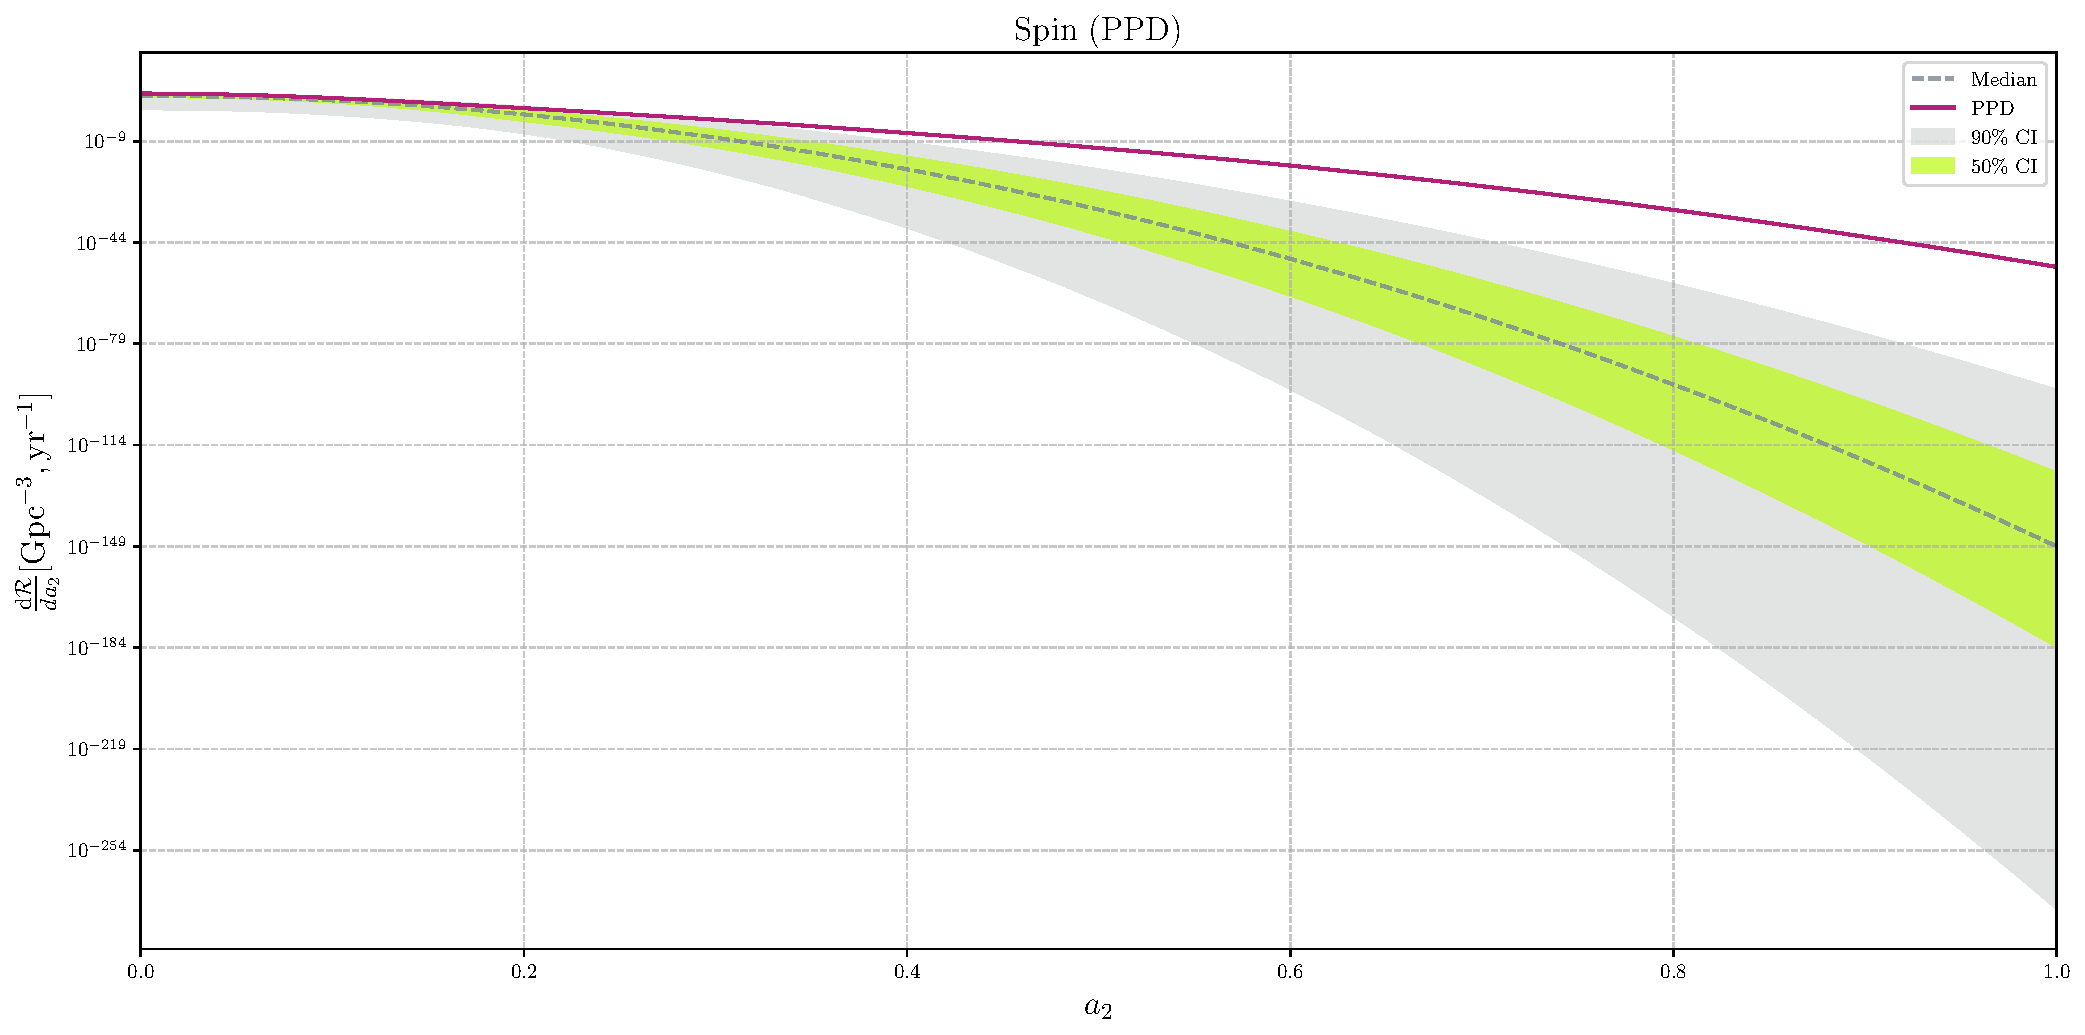
\includegraphics[width=0.7\linewidth]{assets/plots/rate_a_2_ppd_plot.pdf}
    \caption{Posterior Predictive Distribution of Secondary Spin Magnitude}
    \label{fig:ppd-a2}
\end{figure}

\begin{figure}[H]
    \centering
    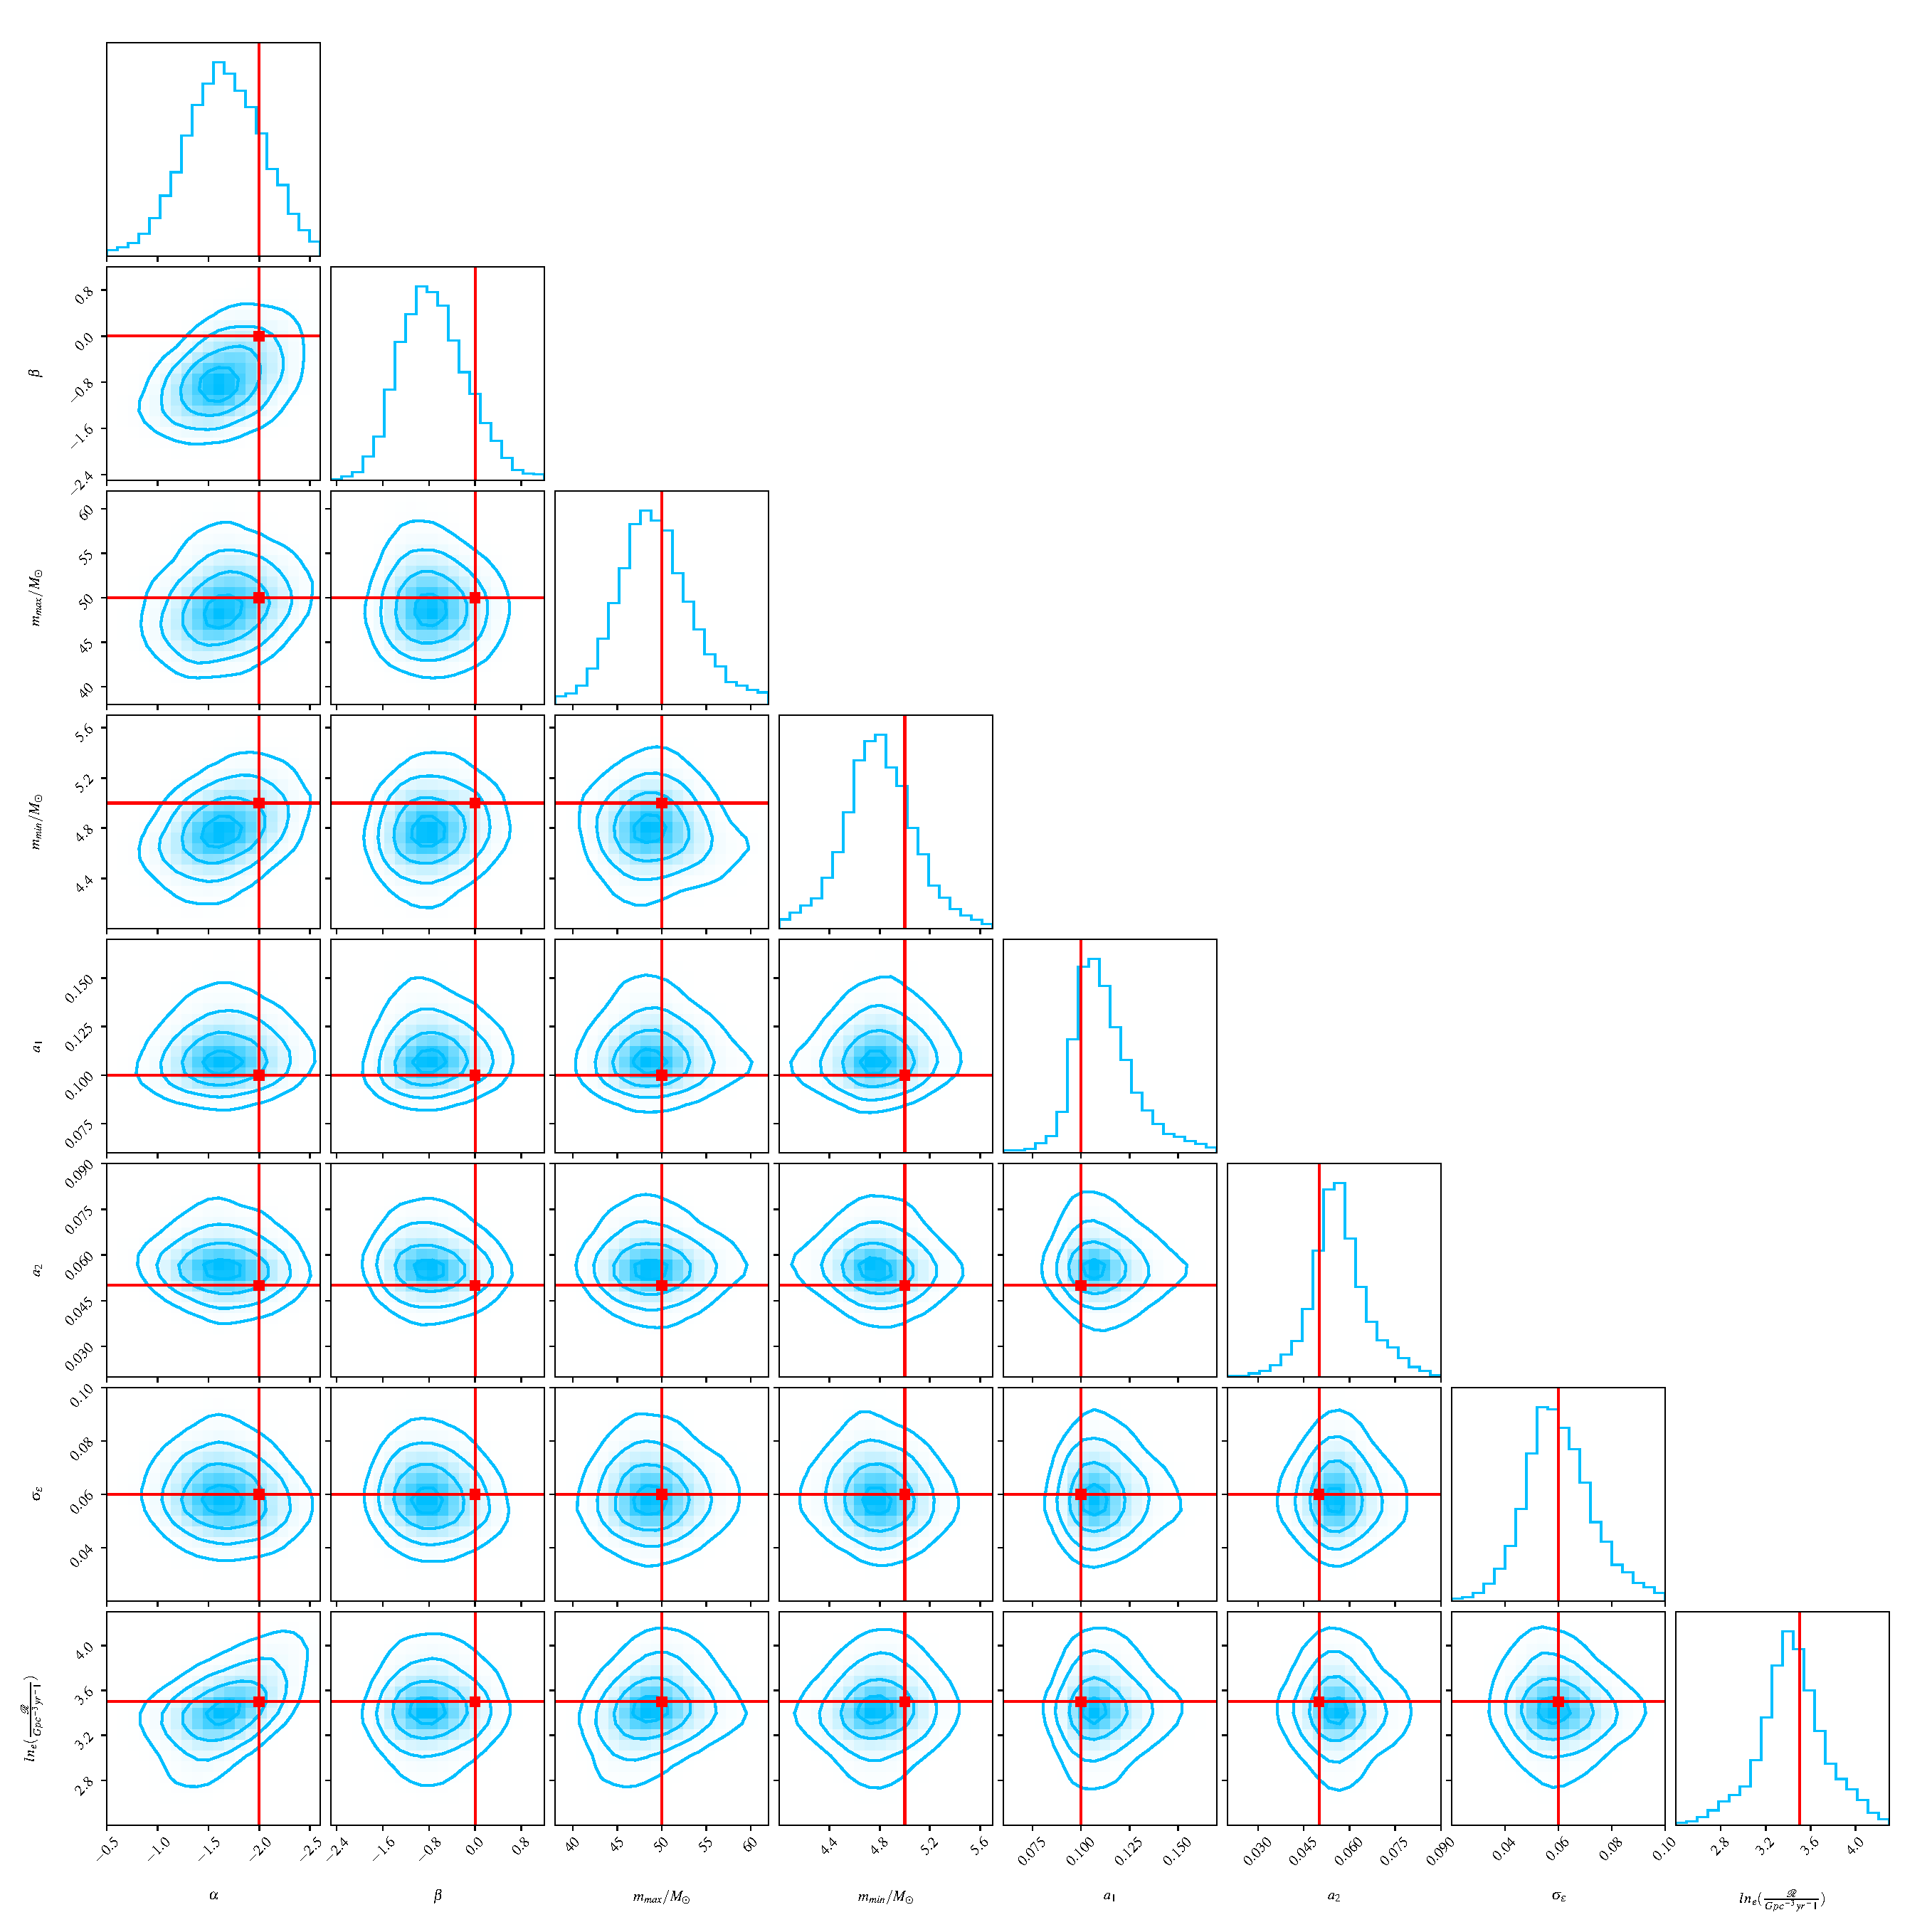
\includegraphics[width=0.7\linewidth]{assets/plots/ecc_spin_corner.pdf}
    \caption{Population Inference of Eccentric Spinning BBHs using Injections and Posteriors Generated by GWKokab}
    \label{fig:ecc_spin_corner}
\end{figure}

\end{frame}

\columnbreak


\section*{Multi-Source Population Inference}

\begin{frame}

\begin{figure}[H]
    \centering
    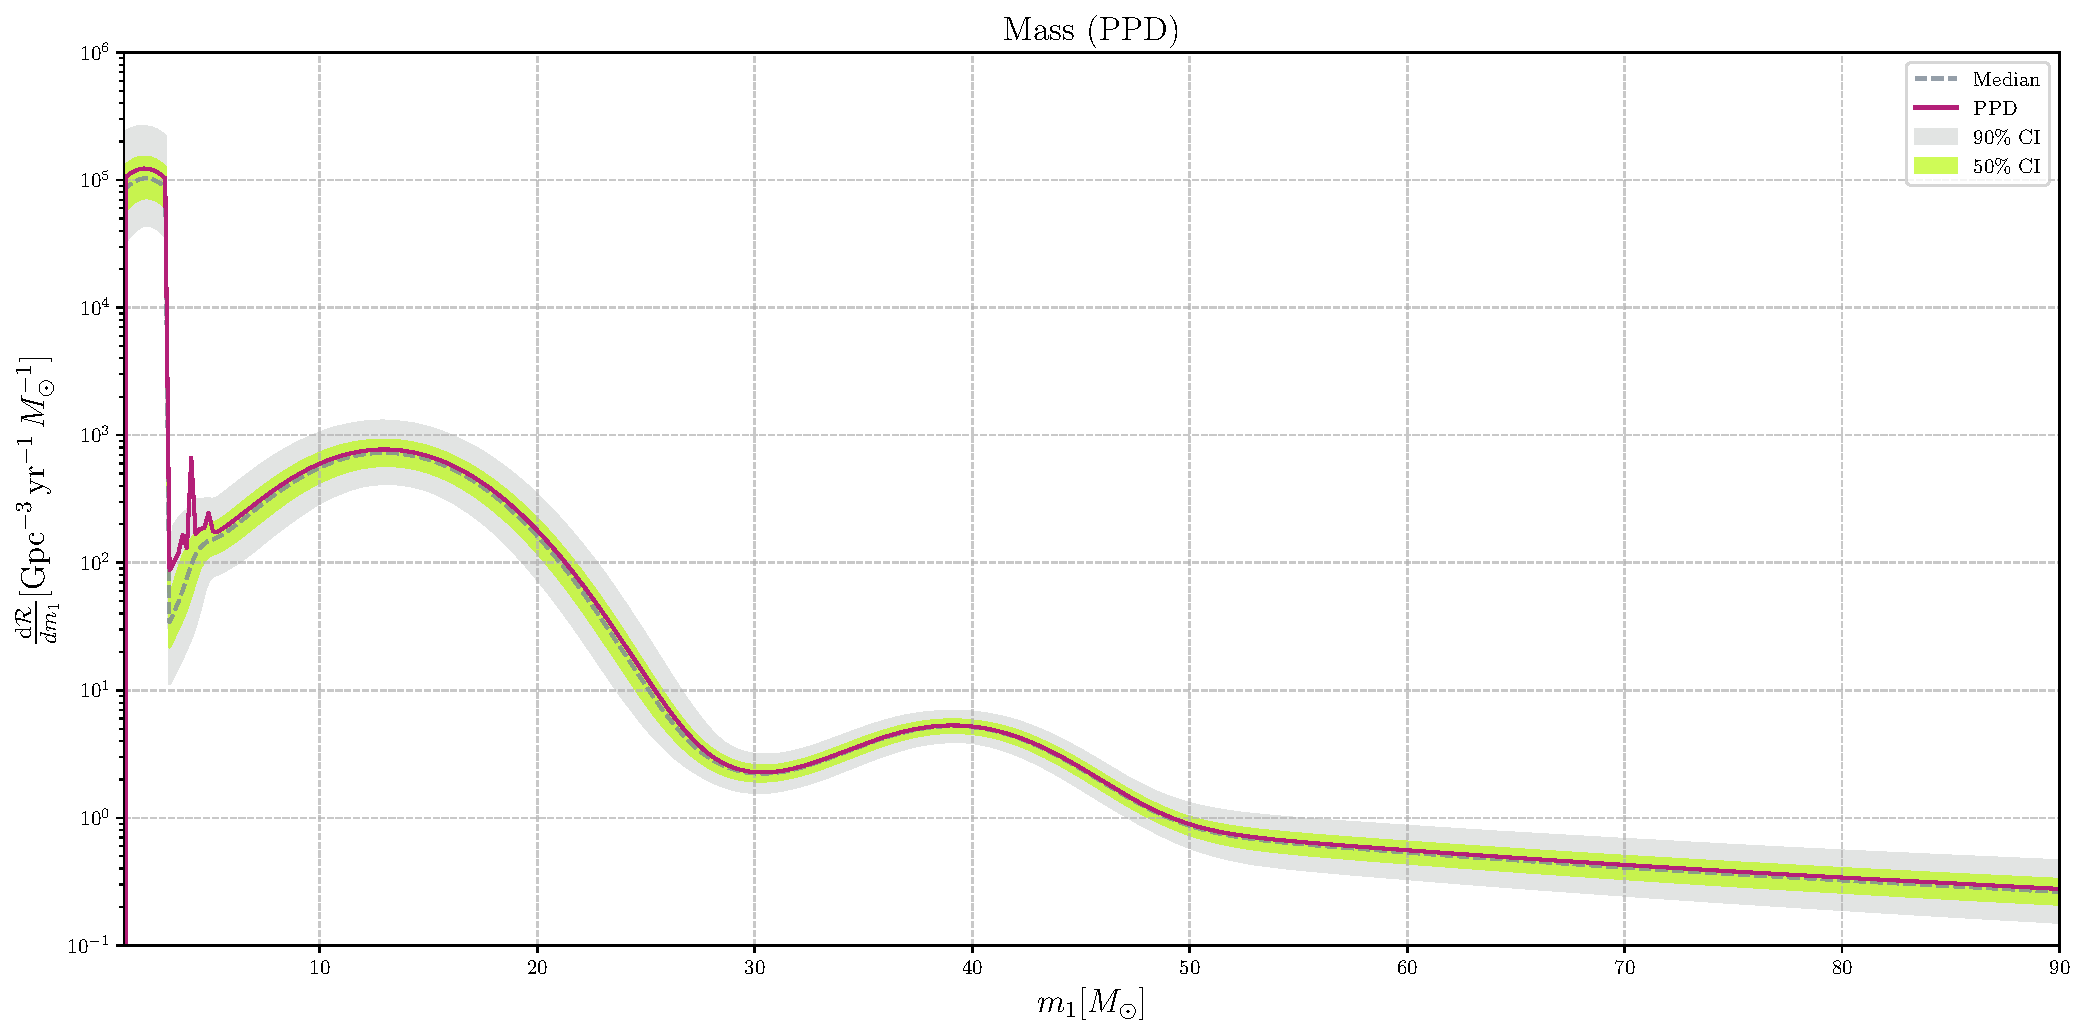
\includegraphics[width=0.7\linewidth]{assets/plots/rate_mass_1_source_ppd_plot.pdf}
    \caption{Posterior Predictive Distribution of Primary Mass}
    \label{fig:ppd-m1}
\end{figure}

\begin{figure}[H]
    \centering
    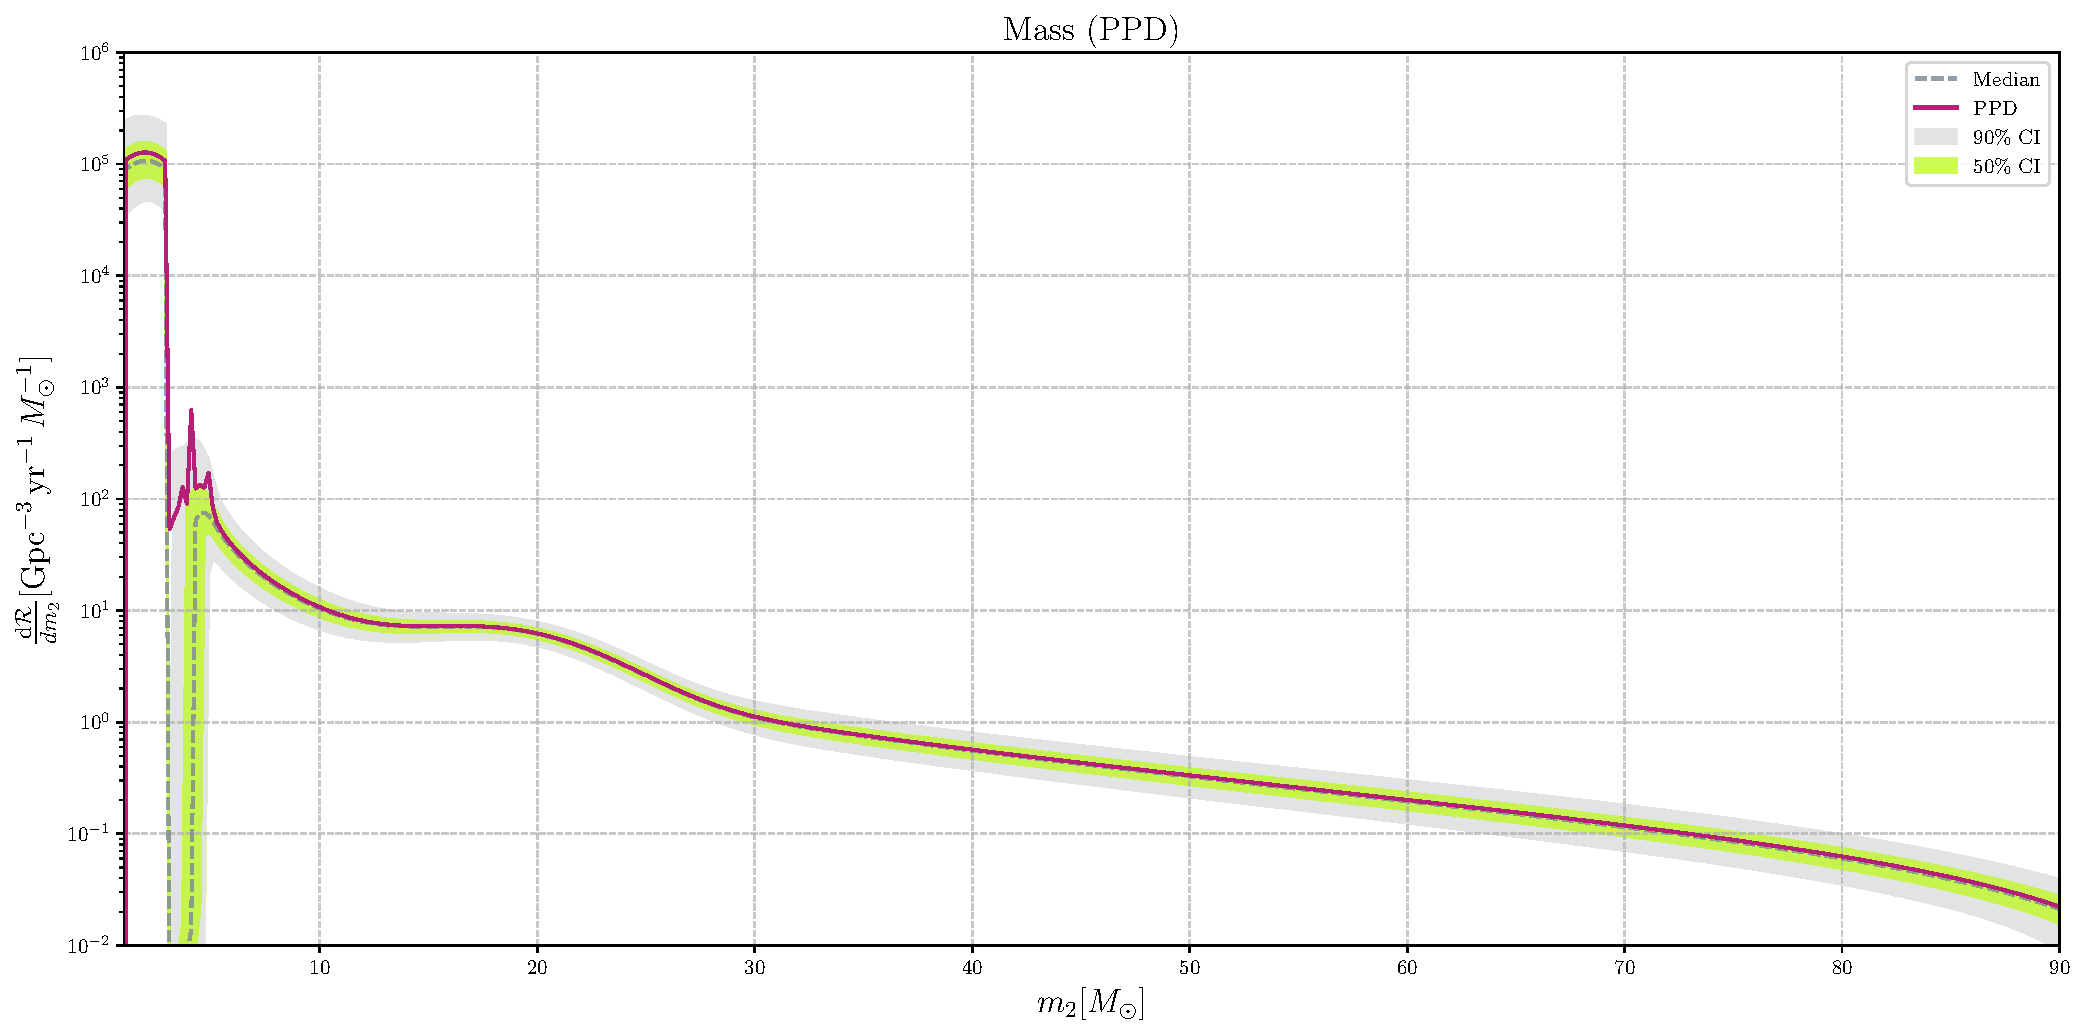
\includegraphics[width=0.7\linewidth]{assets/plots/rate_mass_2_source_ppd_plot.pdf}
    \caption{Posterior Predictive Distribution of Secondary Mass}
    \label{fig:ppd-m2}
\end{figure}

\begin{figure}[H]
    \centering
    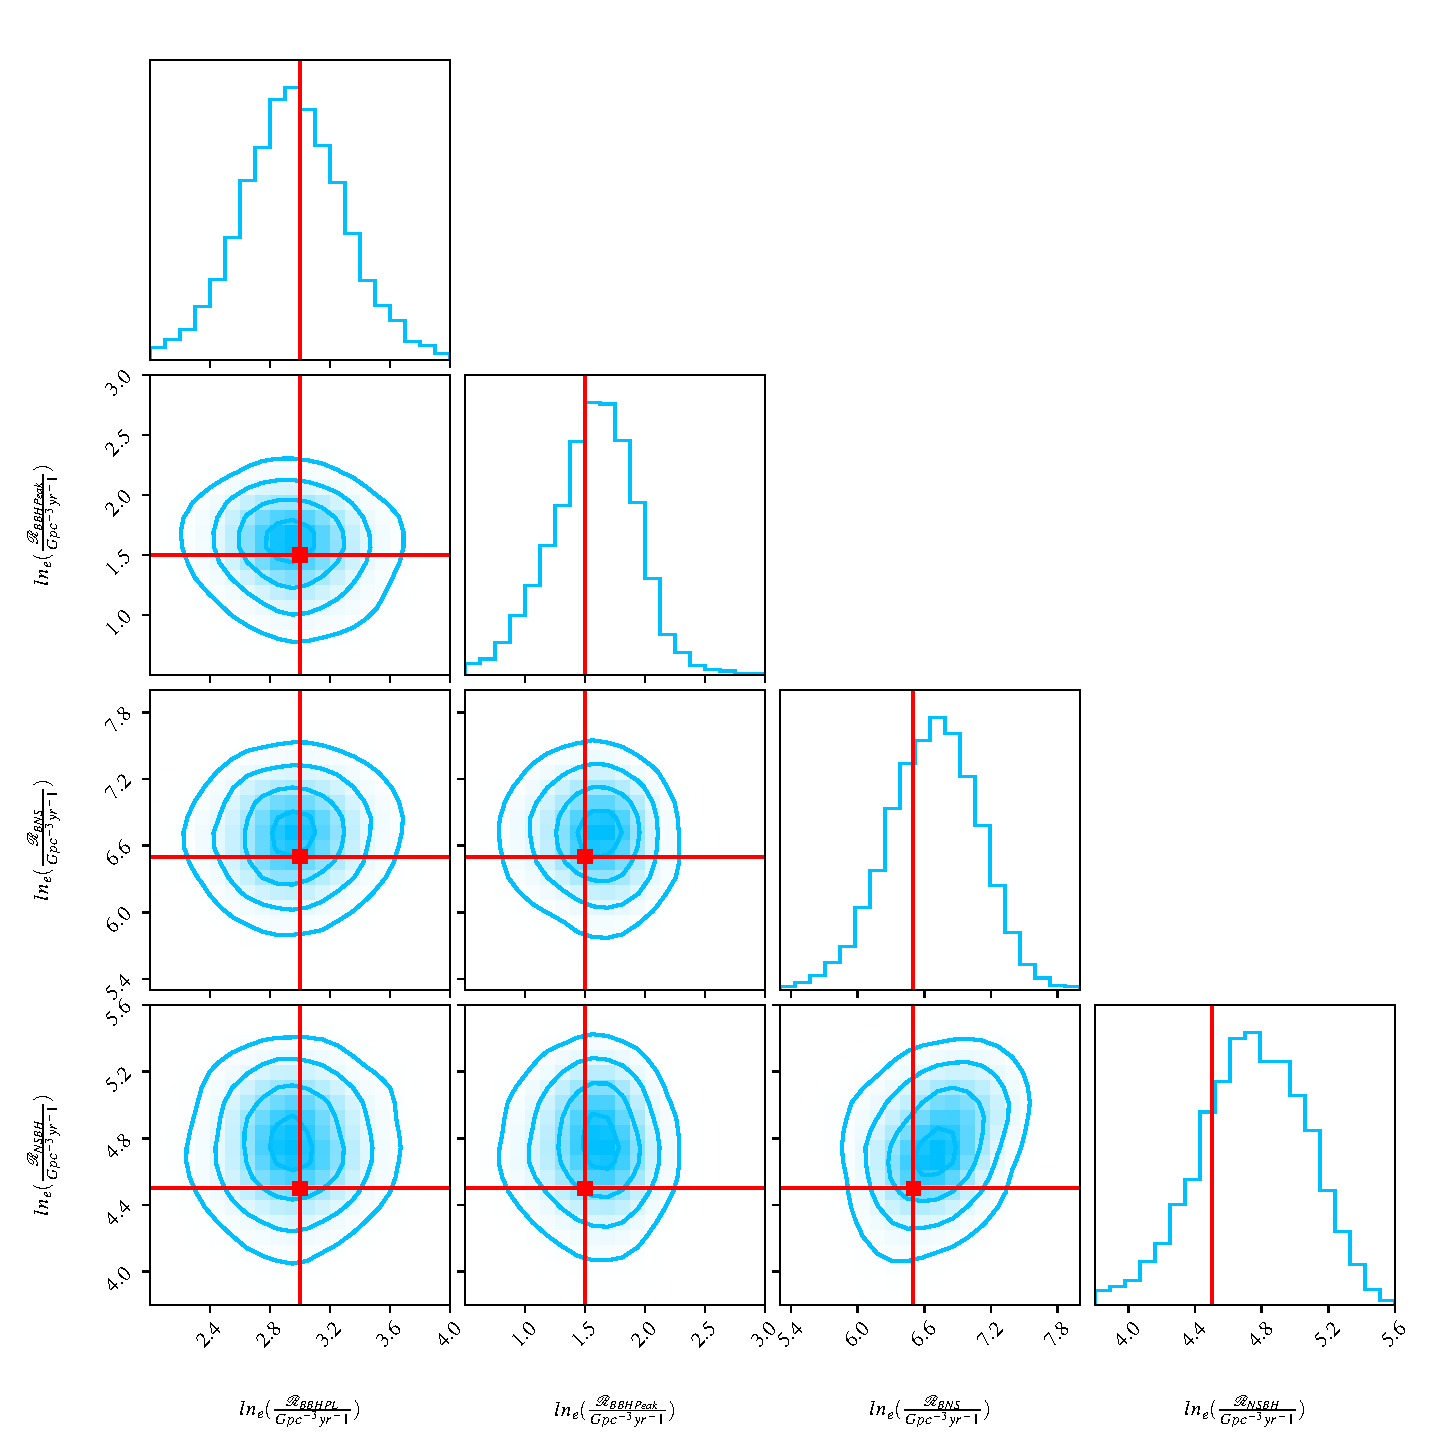
\includegraphics[width=0.7\linewidth]{assets/plots/multi_source_rate.pdf}
    \caption{Rate Recovery of Multi-Source Population}
    \label{fig:multi-source rate recovery}
\end{figure}

\end{frame}

\end{multicols}

% \begin{multicols}{3}

% \begin{figure}[H]
%     \centering
%     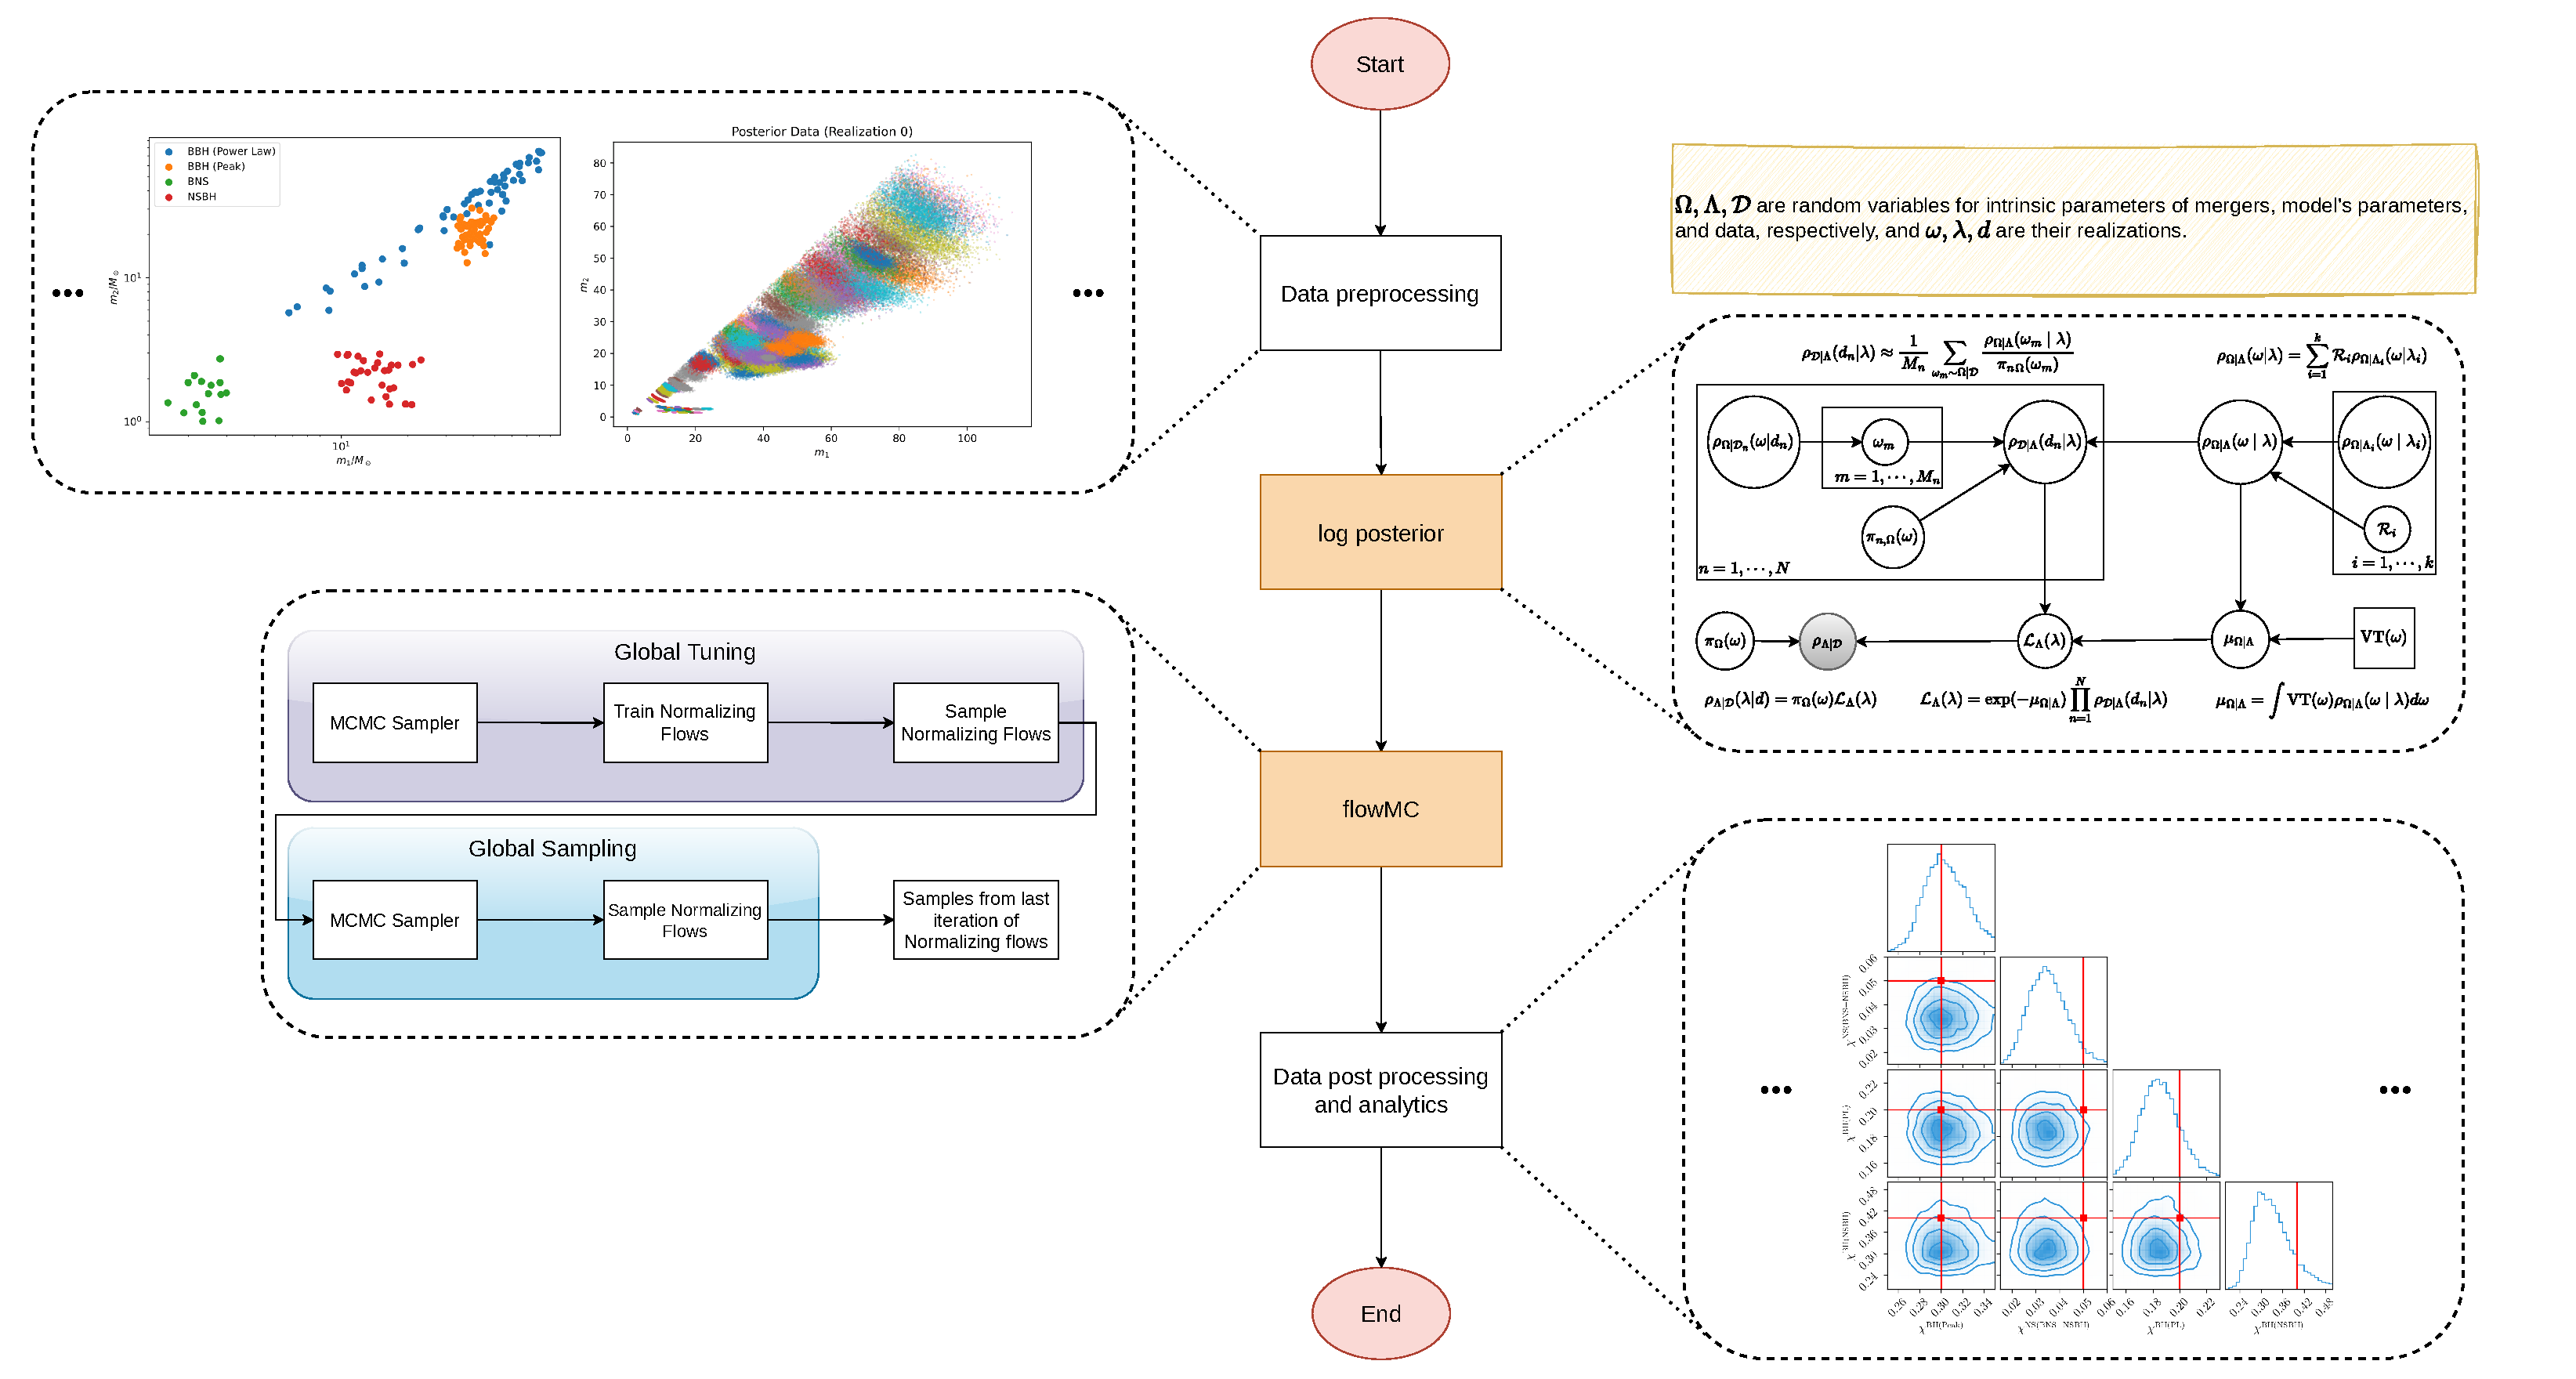
\includegraphics[width=\columnwidth]{assets/plots/post.pdf}
%     \caption{GWKokab's Bayesian Inference Pipeline}
%     \label{fig:plate-likelihood}
% \end{figure}

% \columnbreak

% \begin{figure}[H]
%     \centering
%     
\includegraphics[width=0.4\columnwidth]{assets/logos/qr-code.pdf}
% \end{figure}

% \end{multicols}

\begin{figure}[H]
    \centering
    \begin{minipage}{0.3\linewidth}
        \centering
        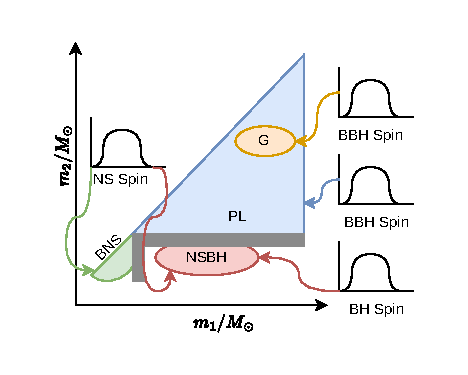
\includegraphics[width=\linewidth]{assets/plots/multisource.pdf}
    \end{minipage}%
    \hfill
    \begin{minipage}{0.5\linewidth}
        \centering
        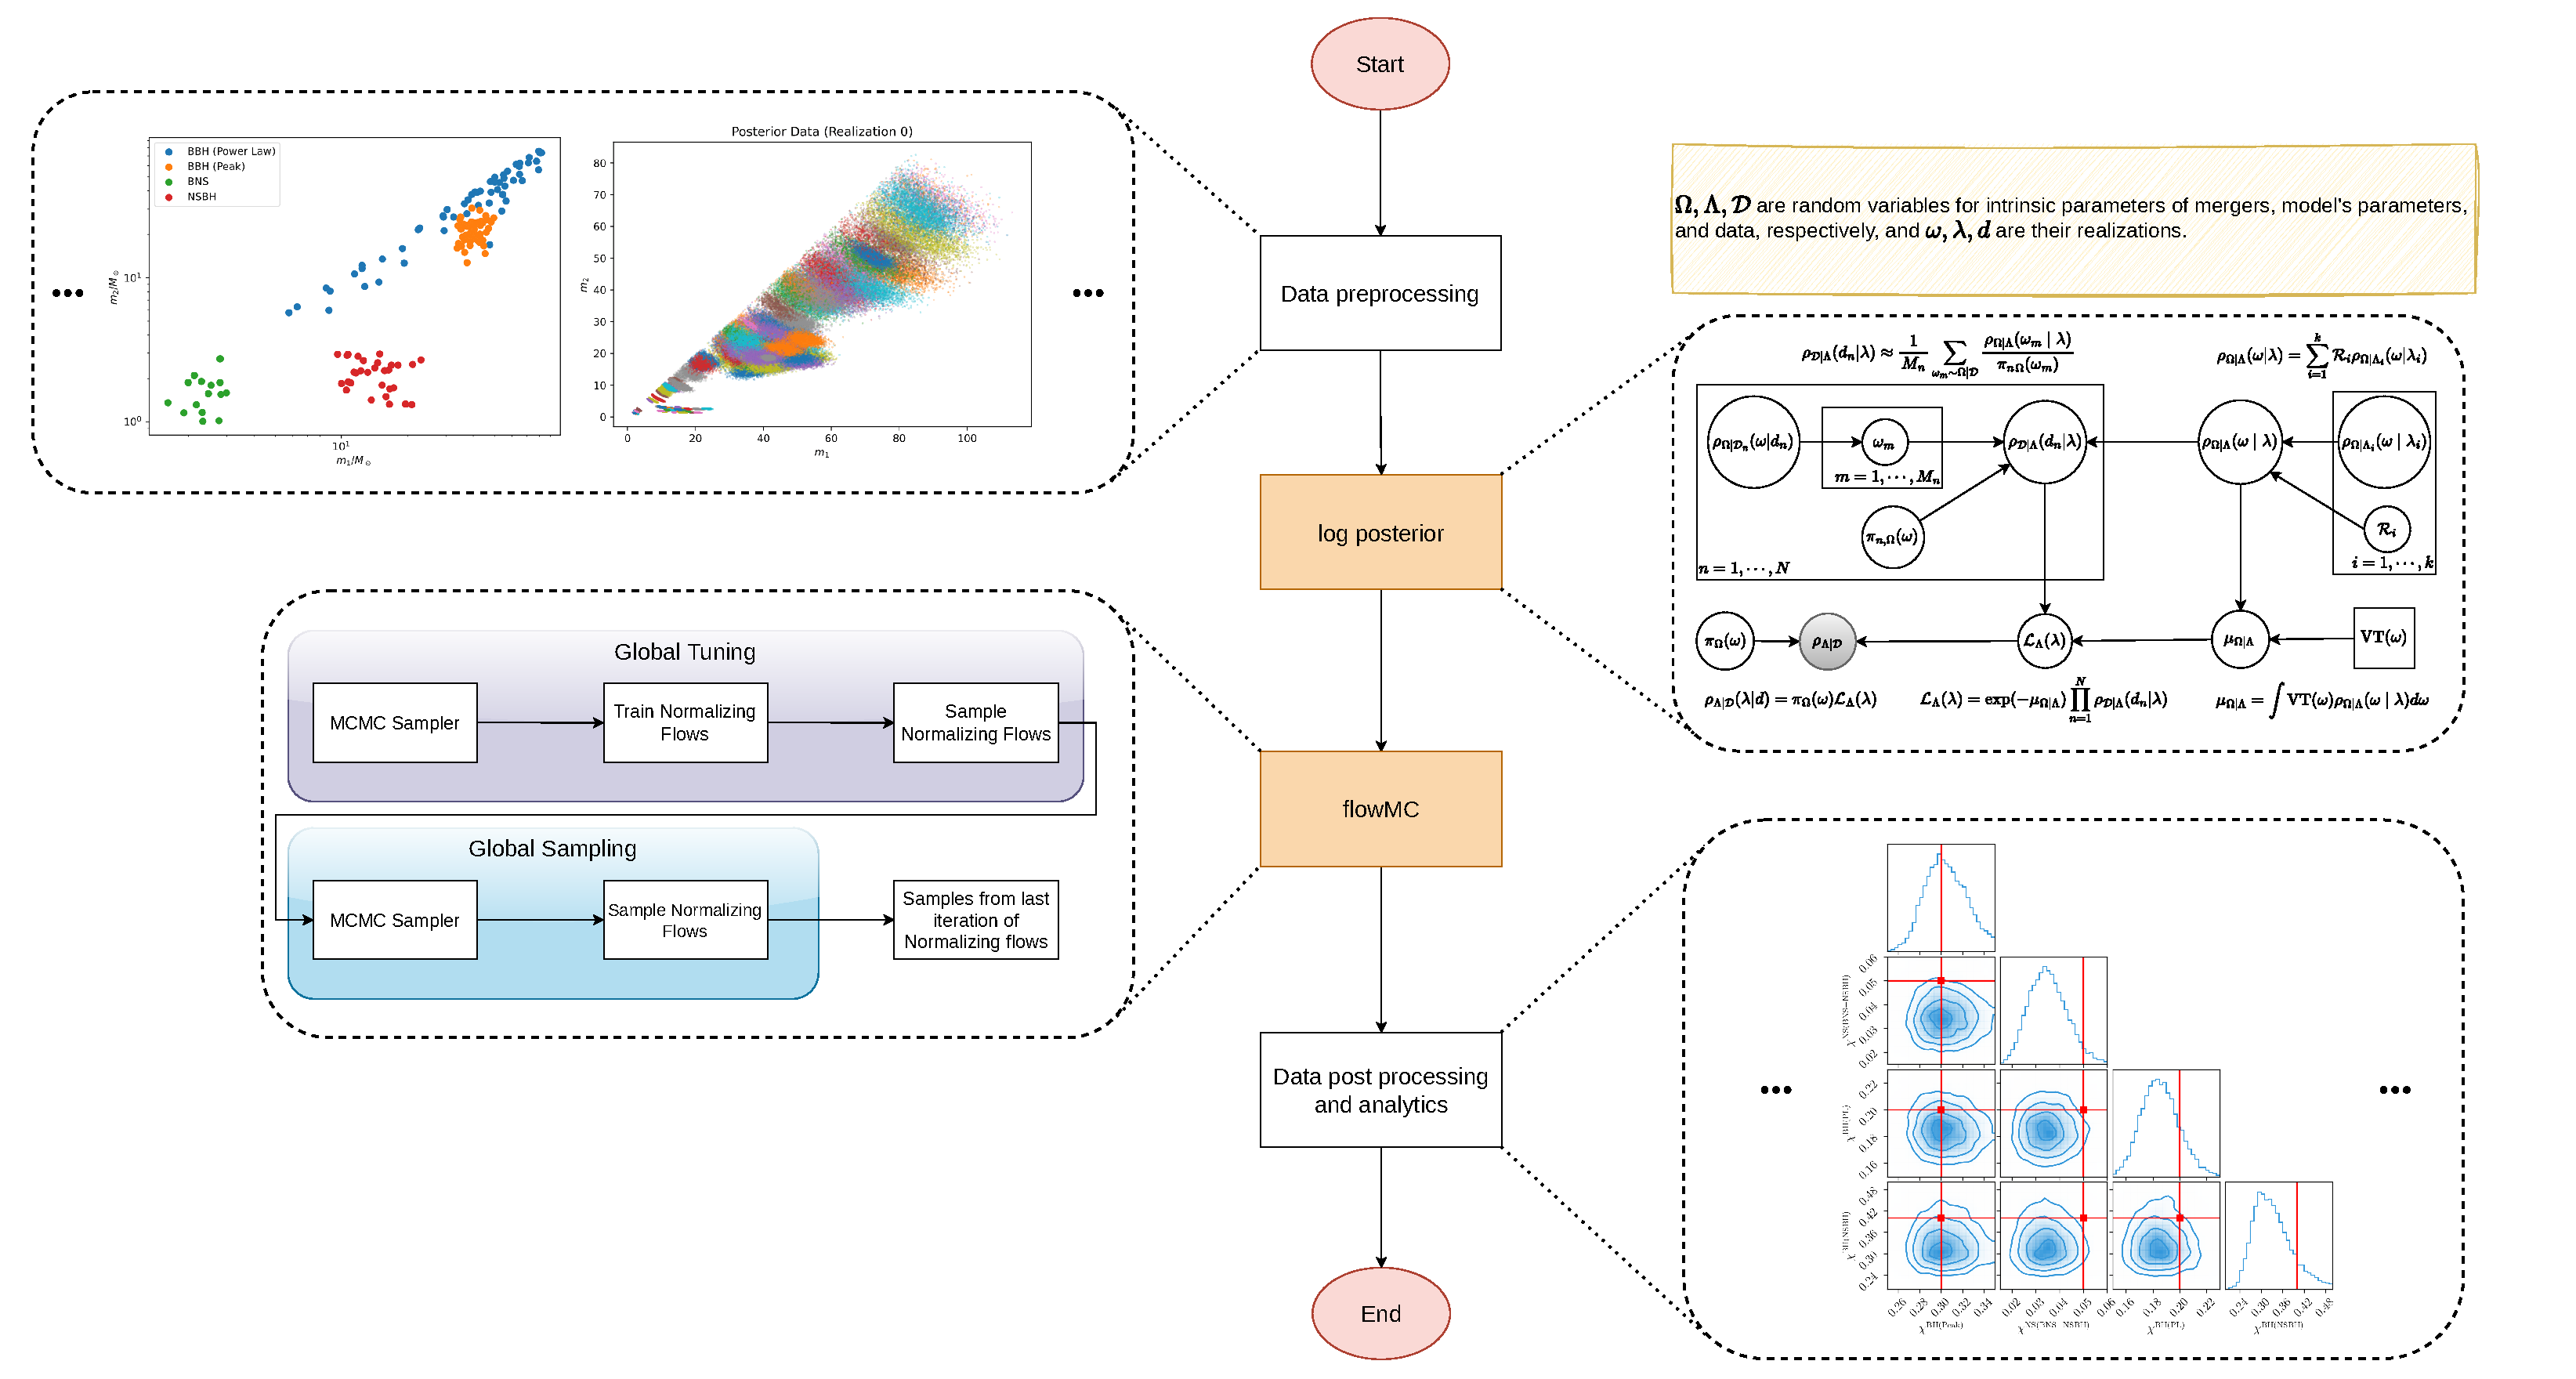
\includegraphics[width=\linewidth]{assets/plots/post.pdf}
    \end{minipage}%
    \hfill
    \begin{minipage}{0.2\linewidth}
        
\includegraphics[width=\linewidth]{assets/logos/qr-code.pdf}
    \end{minipage}
    \caption{GWKokab's Bayesian Inference Pipeline}
    \label{fig:plate-likelihood}
\end{figure}



\begin{multicols}{2}

\section*{Features}

\begin{itemize}
    
\item \textbf{User-Friendly API}: Provides an intuitive and accessible command line interface for creating complex models using simple components.  
\item \textbf{Efficient Sampling Algorithm}: Using a hybrid approach combining normalizing flows with traditional MCMC methods, computations are significantly accelerated compared to pure MCMC techniques.
\item \textbf{Modular Design}: Built with a modular architecture, allowing flexibility and ease of extension for different use cases.

\end{itemize}

\columnbreak

\section*{Future Work}

\begin{itemize}
    
\item \textbf{Scalability Challenges}: Currently, it faces bottlenecks in handling larger datasets, which are actively being addressed.  
\item \textbf{Single-GPU Limitation}: Runs on a single GPU at present, with plans to extend support for multi-GPU execution to enhance performance.
\item \textbf{Binary Neutron Star Analysis} To do the BNS/NSBH analysis with and without the equation of state.

\end{itemize}


\end{multicols}


\end{document}